\section{Cahier des charges}
    \label{sec:cahier}
    % Préciser utilisateur
    % Connais déjà concept arbre d'attaque
    % Responsable sécurité d'une entité
    % Préciser dès l'intro

    % Structure reflète niveau importance

    Comme indiqué dans la section \ref{sec:objectifs}, notre principal objectif est de réaliser un logiciel pouvant assister l'expert en sécurité d'une entreprise. Il devra pouvoir réaliser facilement l'analyse de son système\footnote{La nature du dit système peut être très vaste, allant d'une simple base de donnée à un distributeur de billets.}, en utilisant les arbres d'attaque et de défense décrits dans la section \ref{sec:etat_art}.

    Plusieurs fonctionnalités facilitant l'analyse seront développées:
    \begin{itemize}
        \item Trouver le chemin d'attaque optimal en fonction d'une fonction de synthèse, qui utilisera plusieurs types de valeurs. Nous détaillerons cette fonctionnalités dans la section \ref{sec:fct_synth}
        \item Filtrer l'arbre en fonction d'une fourchette de critères. Voir section \ref{sec:filtre}.
        \item Utiliser des modèles (d'arbres) généraux que l'utilisateur pourra ensuite modifier en fonction de sa situation. Voir section \ref{sec:modele}
    \end{itemize}

    Nous repartirons sur la base d'ADTool pour réaliser notre logiciel, afin de ne pas réécrire l'existant. Toutefois, l'édition des arbres avec ADTool peut être améliorée, afin d'être plus souple et plus pratique. Nous détaillerons nos futures améliorations dans la section \ref{sec:adtoolpp}.

    De plus, bien que ce soit un expert en sécurité qui réalisera l'analyse, celui ci ne sera peut être pas complètement familier avec les arbres d'attaque et de défense. C'est pour cela que notre logiciel intégrera un guide (optionnel) expliquant pas à pas comment réaliser l'analyse. Nous expliquerons son fonctionnement dans la section \ref{sec:guide}

    Pour finir nous décrirons l'architecture de notre logiciel dans la section \ref{sec:archi}.

    \subsection{Fonction de synthèse et chemin optimal}
        \label{sec:fct_synth}

        Avec les outils actuels, il est possible d'utiliser un seul type de valuation à la fois sur un arbre. Pourtant, pouvoir faire une synthèse à partir de plusieurs types peut permettre de rechercher des compromis plus facilement.

        Par exemple, si l'on souhaite rechercher l'attaque la moins coûteuse financièrement, sans pour autant sacrifier le temps passé à réaliser notre attaque, l'on pourrait fournir une fonction telle que \[ synthese(cout, tps) = 2*cout + tps \] 
        Avec cette fonction, une nouvelle valuation de l'arbre serait calculée et on pourra ensuite l'élaguer pour garder uniquement les branches permettant d'atteindre l'objectif avec un coût minimal (selon notre fonction de synthèse). 
        L'arbre épuré sera ensuite affiché, et l'utilisateur qui pourra prendre la décision de l'enregistrer comme un nouvel arbre.

        Afin d'obtenir le plus grand choix de fonctions possibles, nous donnerons à l'utilisateur la possibilité de combiner les types de valuation de façon linéaire, polynomiale, et aussi d'utiliser des fonctions mathématiques \og standards \fg, comme l'exponentielle, le logarithme ou encore les fonctions trigonométriques.

    \subsection{Filtre à critères}
        \label{sec:filtre}

        Une autre fonctionnalité que nous développerons sera le filtre à critères. Les critères consistent en un ensemble de valeurs autorisées pour les types de valuation, et seront gardés uniquement les nœuds respectant ces règles. Cela permettra d'obtenir rapidement les attaques réalisables en fonction de nos ressources, ce qui peut correspondre aux différents attaquants envisagés\footnote{Un étudiant et le Mossad n'auront pas les mêmes moyens financiers ou humains.}.

        Par exemple, supposons qu'il existe trois sous arbres pour atteindre un objectif, avec un coût respectivement de 2596\euro{}, 70333\euro{} et 200\euro{}. Le temps passé à réaliser l'attaque dure 1, 2 et 3 semaines. On voudrait garder uniquement les attaques qui coûtent moins de 30000\euro{}, et qui prennent entre une et deux semaines. Notre filtre supprimera donc les sous arbres B et C, pour garder uniquement le A.

        Contrairement à la fonction de synthèse, le nombre de chemins possibles restant n'est pas connu à l'avance. On peut très bien obtenir zéro chemin possible, ou au contraire en obtenir une infinité.

        \`A l'instar des fonctions de synthèse, le résultat sera affiché à l'utilisateur qui décidera ensuite de ce qu'il en fera.

    \subsection{Modèles généraux}
        \label{sec:modele}

        L'utilisateur pourra se baser sur des modèles déjà réalisés lors d'autres analyse. Par exemple, pour rester dans notre cas d'étude, on pourrait partir d'un modèle d'attaque générique à n'importe quel réseau de transport public, pour ensuite l'éditer afin de correspondre à la situation rennaise.

        Notre logiciel intégrera divers arbres génériques, mais l'utilisateur pourra aussi en importer depuis d'autres sources (internet, clé usb, etc.). Notre logiciel étoffera sa collection de modèles à chaque nouveau modèle importé par l'utilisateur.

        L'utilisateur sera aussi capable de créer ses propres modèles, pour s'en resservir dans d'autres de ses analyses, ou encore pour les publier sur son site internet. Ainsi, un pourrait imaginer à terme un site web regroupant des milliers de modèles réalisés par un réseau d'experts en sécurité.

    \subsection{Amélioration d'ADTool}
        \label{sec:adtoolpp}

        Bien qu'ADTool soit déjà très complet, nous avons identifié plusieurs fonctionnalités qui rendraient la manipulation des arbres plus aisée:
        \begin{itemize}
            \item Une fonction de couper / copier / coller d'arbres et de sous arbres.
            \item Réaliser des glisser / déposer d'arbres et de sous arbres.
            \item Importer et exporter des arbres dans un grand nombre de formats différents.
            \item Permettre la représentation d'un arbre avec plusieurs types de valuation à la fois.
        \end{itemize}

    \subsection{Guide}
        \label{sec:guide}

        L'utilisateur n'étant pas nécessairement complètement familier avec les arbres d'attaque défense, le guide lui permettra de comprendre rapidement comment réaliser ses arbres, et comment il doit réaliser son analyse.

        Notre guide lui fera suivre une méthode générique~\cite{methode_analyse}, découpée en différentes étapes. Une fois que l'une d'entre elle sera complétée, le guide passera à l'étape suivante et expliquera précisément à l'utilisateur comment la réaliser.
        Le guide prendra la forme d'un \og journal de quête \fg, ce qui lui permettra de garder une trace des étapes déjà réalisées.
        
        Notons que nous ne voulons pas forcer l'utilisateur à suivre une méthode en particulier, et le guide sera donc désactivable afin de ne pas importuner les personnes voulant faire autrement.

    \subsection{Architecture}
        \label{sec:archi}

        L'analyse d'un système sera sauvegardée sous forme de projet. Celui ci contiendra différents arbres utilisé pour l'analyse, ainsi qu'une bibliothèque de modèles que l'utilisateur pourra reprendre à tout moment pour créer un nouvel arbre (groupe "Fichier Projet" de la figure \ref{fig:archi}). 

        \begin{figure}
            \begin{center}
                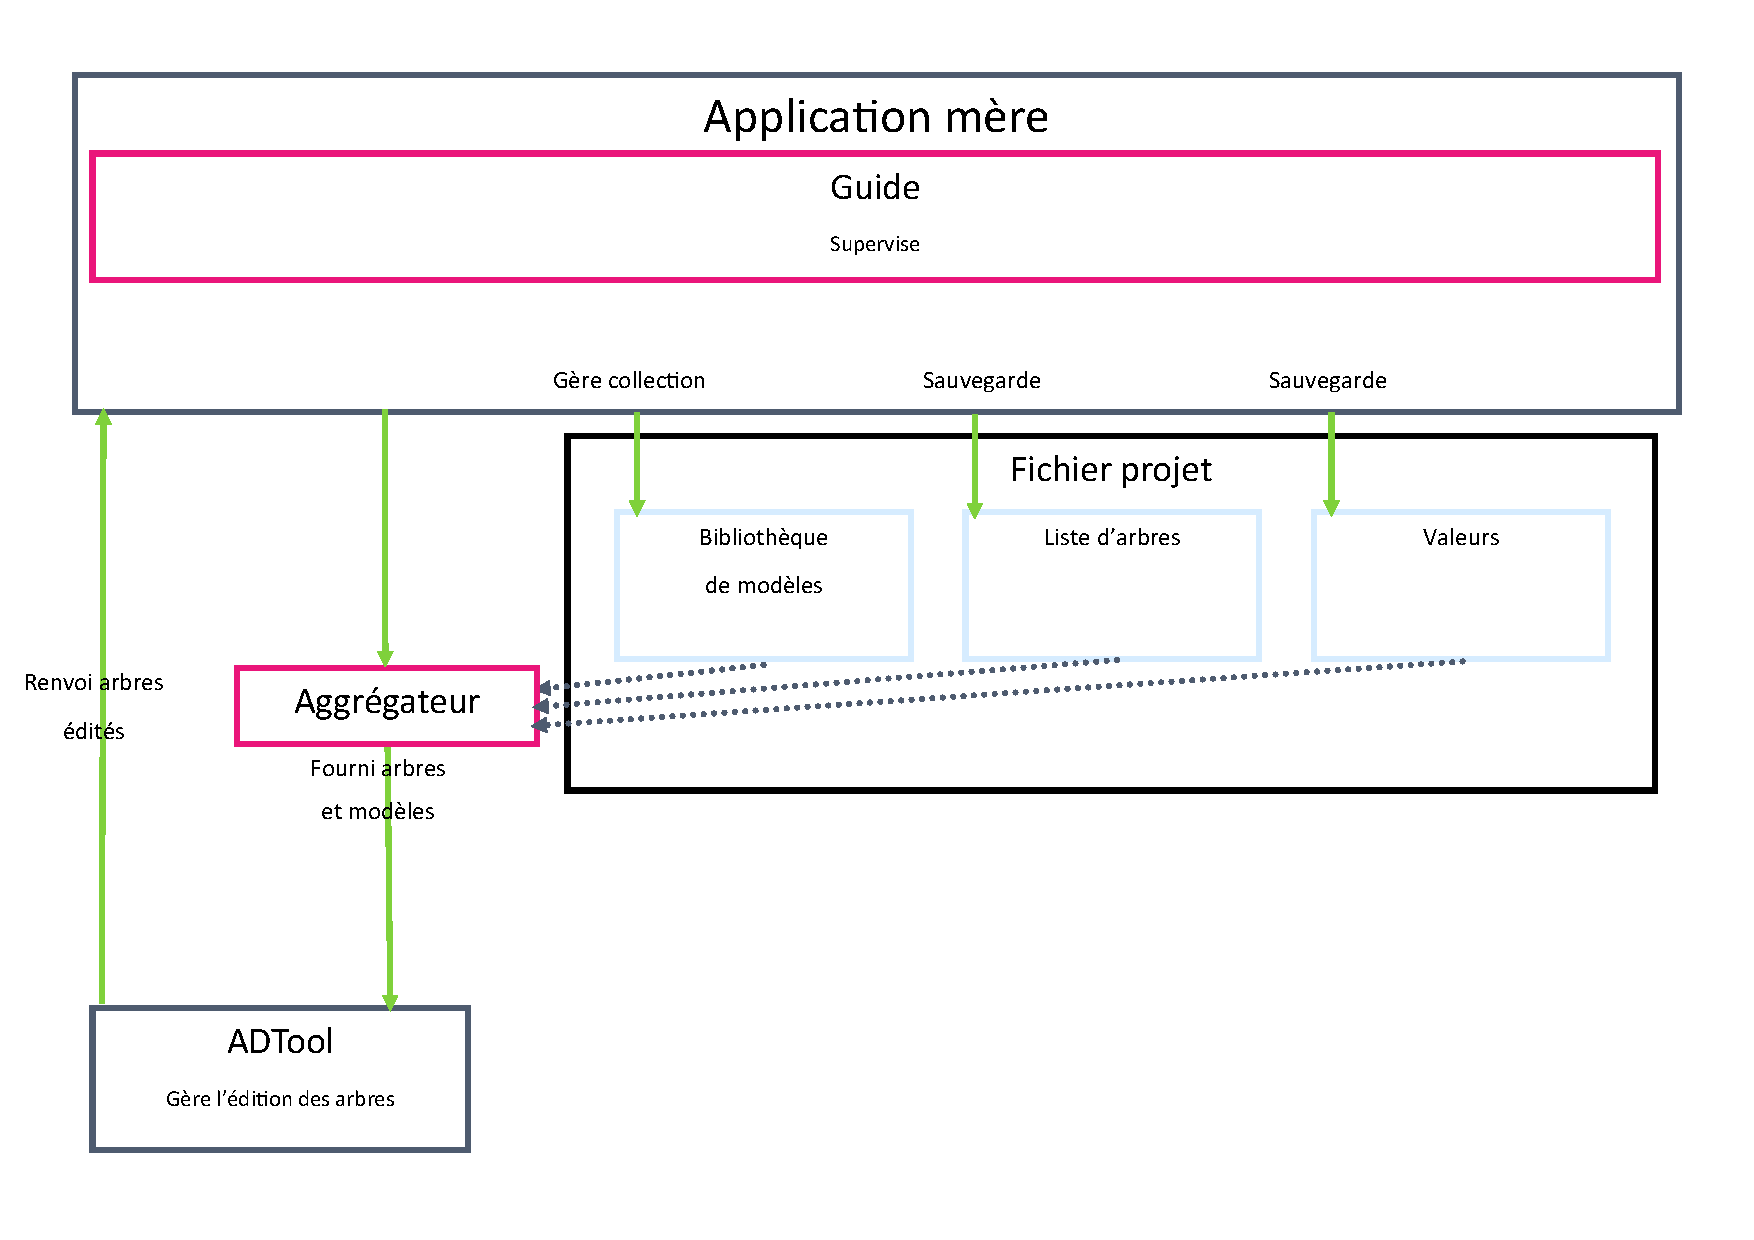
\includegraphics[width=1\textwidth]{figure/archi.pdf}
            \end{center}
            \caption{Différents modules graviteront autour d'ADTool pour atteindre nos objectifs.}
            \label{fig:archi}
        \end{figure}

        Cette bibliothèque sera préchargée avec différents modèles à la création du projet. En effet, l'utilisateur devra répondre à une série de questions, qui permettra de sélectionner un sous-ensemble des modèles de la bibliothèque de notre logiciel.

        Comme indiqué par la figure \ref{fig:archi}, ADTool sera un composant de notre application. Il servira à la fois à la visualisation et à l'édition des arbres. Ce choix sera détaillé dans la section \ref{sec:outils}.

        La fonction de synthèse et le filtre seront deux modules différents de l'application. Ils prendront en entrée un arbre du fichier projet (et leurs autres paramètres respectifs), et enverront le résultat à ADTool pour affichage. L'utilisateur décidera ensuite ce qu'il fera de l'arbre généré.

        Le guide supervisera l'ensemble de l'application, et devra fournir des informations et consignes pertinentes à l'utilisateur.

        Une ébauche de l'interface se situe figure \ref{fig:interface}. Notons que le guide n'y figure pas, puisqu'il ne sera pas affiché en permanence pour ne pas surcharger l'interface. Il s'agira plutôt d'une fenêtre dédiée qui pourra être ouverte et fermée au besoin.

        \begin{figure}
            \begin{center}
                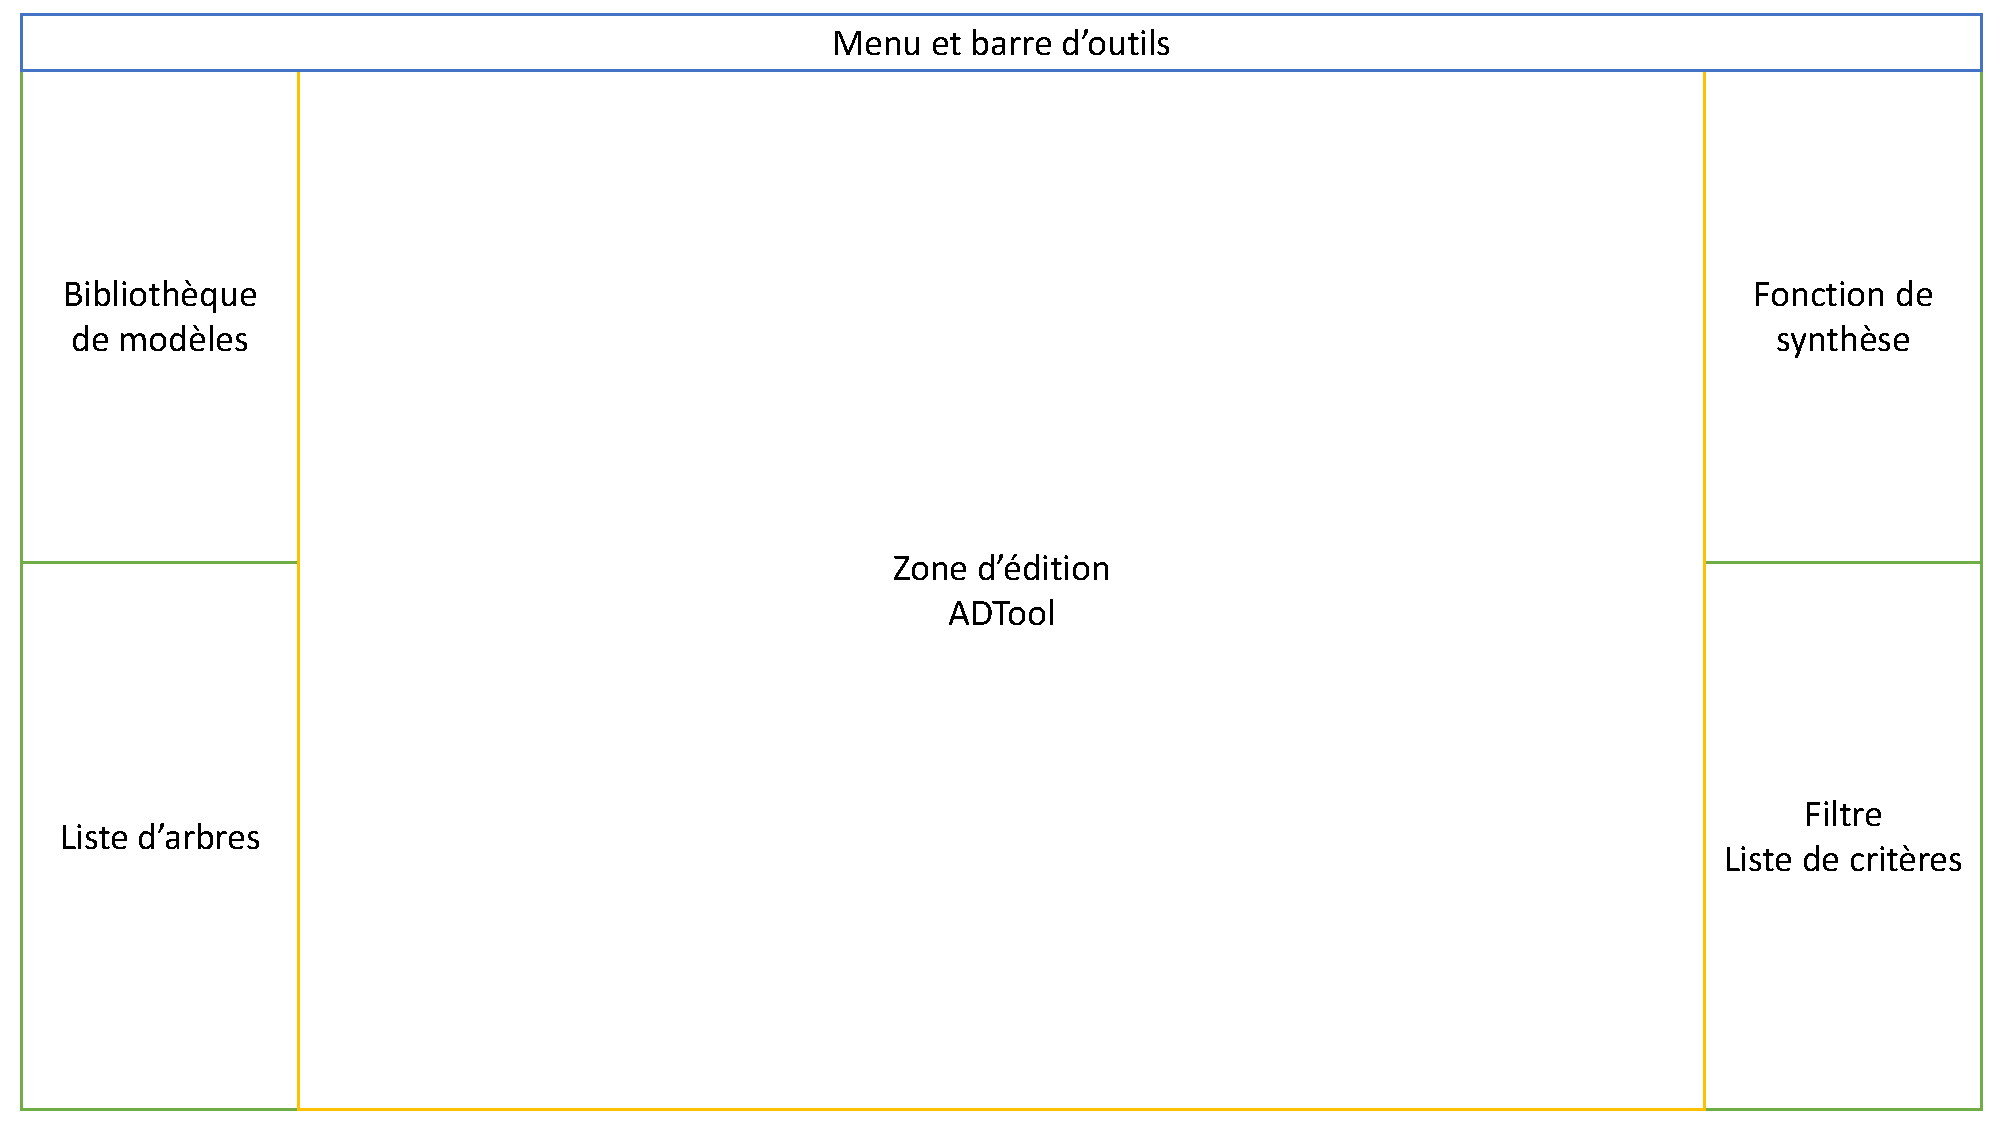
\includegraphics[width=1\textwidth]{figure/interface.pdf}
            \end{center}
            \caption{L'interface sera gardée au plus simple.}
            \label{fig:interface}
        \end{figure}